\documentclass[a4paper,10pt,titlepage]{article}
% PREUMBULUM
\usepackage[utf8]{inputenc}
\usepackage[T1]{fontenc}

\usepackage{a4wide} 

% Használjunk inkább Arial betűtípust:
%\usepackage{times}
\renewcommand{\rmdefault}{phv} % Arial
\renewcommand{\sfdefault}{phv} % Arial

\usepackage[magyar,english]{babel}

% Forráskódoknak:
\usepackage{listings}

% Tartalomjegyzék:
\usepackage{tocbibind}

\usepackage[usenames,dvipsnames]{color}

% Hogy legyen képünk:
\usepackage{graphicx}

%###############################################################################
\newcommand{\szerzo}{Nádudvari György}
\newcommand{\szerzomail}{ulqp9p@gmail}
\newcommand{\cim}{Rendszermodellezés - 2. gyakorlat \\ Vizuális adatelemzés}
\newcommand{\targy}{rendszermodellezés, vizuális adatelemzés}
\newcommand{\kulcsszavak}{rendszermodellezés, vizuális adatelemzés, adattisztítás, Mondrian, TPC, TPC-C}

\usepackage{hyperref}
\hypersetup{
    unicode=true,
    colorlinks=true,
    linkcolor=RoyalBlue,
    citecolor=RoyalBlue,
    filecolor=RoyalBlue,
    urlcolor=RoyalBlue,
    pdftitle={\cim},        % title
    pdfauthor={\szerzo},    % author
    pdfsubject={\targy}, % subject of the document
    pdfcreator={},   % creator of the document
    pdfproducer={LaTeX, TexMaker},    % producer of the document
    pdfkeywords={\kulcsszavak},    % list of keywords
}

\usepackage{url}

% Táblázatoknak:
\usepackage{colortbl}

% Ha kell matek:
\usepackage{amssymb,amsmath}

\usepackage{subfig}
\usepackage{verbatim} % Hogy lehessen blokkkommentezni

% Egymás melleti képekhez:
\usepackage{subfig}

\usepackage{ftsrgtemplate}

\setlength{\parindent}{12pt} % magyar nyelvű dokumentumokban jellemző
\setlength{\parskip}{0pt}    % magyar nyelvű dokumentumokban jellemző

%###########################################
% Saját eszközök:
%
\definecolor{todobgszin}{rgb}{0.64,0.78,0.22}
\definecolor{todofrszin}{rgb}{0.00,0.50,0.00}

%\newcommand{\todo}[1]{\fcolorbox{todofrszin}{todobgszin}{\emph{TODO: #1}}}
\newcommand{\angolul}[1]{\foreignlanguage{english}{#1}}

\newcommand{\todo}[1]{
    \vfill
    \begingroup % Csinálunk egy csoportot, hogy az identálás csak erre vonatkozzon
        \setlength{\parindent}{0cm} % Beállítjuk, hogy teljes szélességű legyen a dobozunk a bekezdéstől függetlenül
        \fcolorbox{todofrszin}{todobgszin}{
            \parbox{\textwidth}{
                \vskip10pt
                \leftskip10pt
                \rightskip10pt
            
                \emph{TODO: #1}
  
                \vskip10pt
            }
        }
    \endgroup
    \vfill
}


%###############################################################################
\newcommand{\oszlopnev}[1]{\texttt{#1}}
\newcommand{\menuelem}[1]{\emph{#1}}

\newenvironment{sajat_itemize}
{
	\begin{itemize}
	\setlength{\itemsep}{0pt}
}
{
	\end{itemize}
}

\begin{document}
% Dokumentumtörzs

\selectlanguage{magyar}

% Címoldal:
\begin{titlepage}

\title{\colorbox{ftsrg_color}{\parbox{\textwidth}{%
  \vskip40pt
  \leftskip10pt\rightskip10pt
  \center{\color{white}{Rendszermodellezés - 2. gyakorlat \\ Vizuális adatelemzés}}
  \vskip40pt
 }
}}
\author{\szerzo \\ < \szerzomail >}
\date{\today}

\end{titlepage}
\maketitle

% Nem akarom, hogy megjelenjen a tartalomjegyzékben a Tartalomjegyzék:
\section*{Tartalomjegyzék}
\makeatletter
\@starttoc{toc}
\makeatother

\newpage

\section{Bevezetés}

A gyakorlat célja, hogy nagy vonalakban bemutassuk a vizuális adatelemzést és az ahhoz kapcsolódó előkészületeket, használható alkalmazásokat.

\todo{Bővíteni!}

%------------------------------------------------------------------------------
\section{Benchmarking}
\subsection{Mik azok a benchmarkok?}

A benchmarkok olyan részletesen specifikált, dokumentált, megismételhető mérések, amelyek segítségével hardver- és/vagy szoftverkonfigurációk teljesítményeinek összehasonlítását hivatottak segíteni. A benchmark környezet specifikációjában rögzített a

\begin{sajat_itemize}
\item hardver komponensek listája,
\item szoftver komponensek listája,
\item üzemviszonyok,
\item ütemezés,
\item dokumentáció.
\end{sajat_itemize} 

\subsection{A TPC benchmarkok}
A TPC benchmarkokat a nonprofit \textit{Transaction Processing Performance Council} dolgozta ki, amelyek főleg web és adatbázis rendszerek teljesítményét hivatottak mérni.

További információkat a szervezet honlapján (\url{http://www.tpc.org}) találhatunk.

\subsection{A TPC-C benchmark}
A TPC-C benchmark egy összetett OLTP (On-line Transaction Processing) benchmark, amely különböző típusú és komplexitású konkurens tranzakciók percenkénti számát méri (tpmC). A tranzakciók lefutási idejére rögzített felső korlát van.

A mérési környezet része egy mintaadatbázis, amely ügyfeleket és megrendeléseket tartalmaz. A mérés kialakításánál igyekeztek ACID körülményeket, és a felhasználók gondolkodási idejét is szimulálni. A mért adatok az áteresztőképesség (tpmC) és a hatékonyság (ár/tpmC). 

A segédlet további részében ezeket az eredményeket fogjuk felhasználni.
 
%------------------------------------------------------------------------------
\section{Adattisztítás}

Általában minden adatelemzést megelőz az adatok tisztítása.

\todo{Bővíteni!}

\subsection{Manuális adattisztítás}

Kisméretű adathalmaz esetén akár kézzel is megtisztíthatjuk azt. Ehhez csak ismernünk kell az adatok jelentését, hogy miből származnak, milyen formátumban állnak rendelkezésre az egyes mezők. Egyszerűsödik a munka, ha olyan elrendezésben érhetőek el, hogy azt egy táblázatkezelő alkalmazásba tudjuk importálni. 

Mostani példánkban a TPC-C eredményeinek átalakításán megyünk végig, áttekintve ezzel az adattisztítás fontosabb lépéseit. Ezek az eredmények letölthetőek a TPC honlapjáról: \url{http://www.tpc.org/downloaded\_result\_files/tpcc\_results.txt}

\todo{Írjuk-e ezt le részletesen, lépésről-lépésre?}

\Aref{fig:tpc_raw}.~ ábrán látható az adathalmazunk, miután importáltuk kedvenc táblázatkezelőnkbe.

\begin{figure}[h!]
\centering
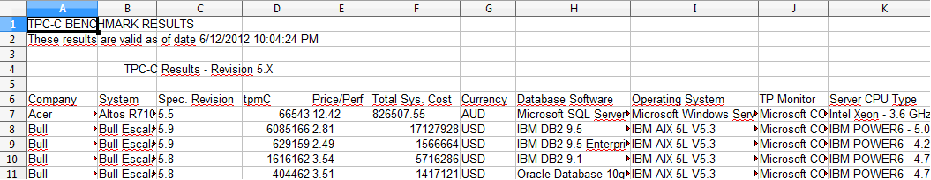
\includegraphics[width=0.90\textwidth]{figures/tpc_raw.png}
\caption{A tisztítatlan adathalmaz importálás után \label{fig:tpc_raw}}
\end{figure}

A tisztítás fontosabb lépései:

\begin{sajat_itemize}
\item importálás táblázatkezelőbe
\item felesleges sorok eltávolítása
\item felesleges oszlopok eltávolítása (itt pl. spec. revision, withdraw stb.)
\item tizedespont vs. vessző átalakítások a számokat tartalmazó cellákban
\item új származtatott oszlopok felvétele (itt pl. Price/Perf (USD) és Total Sys. Cost (USD))
\item adatok aggregálása (itt pl. Database Software, Operating System)
\item exportálás (esetünkben tabulált értékek, hogy a később bemutatásra kerülő Mondriánba tudjuk importálni)
\end{sajat_itemize}

\Aref{fig:tpc_cleaned}.~ ábrán látható a tisztított adathalmazunk.

\todo{Mivel főleg nem látható, ezért több, jobb képet csinálni!}

\begin{figure}[h!]
\centering
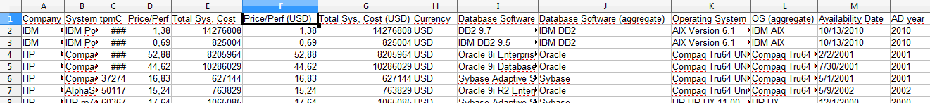
\includegraphics[width=1.00\textwidth]{figures/tpc_cleaned.png}
\caption{A tisztítatlan adathalmaz importálás után \label{fig:tpc_cleaned}}
\end{figure}

\subsection{Automatikus adattisztítás}

Nagyobb méretű adathalmaz esetén nem alkalmazható a kézi tisztítás, ehelyett ilyenkor céleszközöket használunk.

\todo{Bővíteni!}

\colorbox{todobgszin}{\parbox{\textwidth}{%
  \vskip40pt
  \leftskip10pt\rightskip10pt
  
  \begin{sajat_itemize}
      \item nagy adathalmaza, esélytelen a kézi tisztítás
      \item R vagy egyéb script/programozási nyelv alkalmazása
      \item KNIME
  \end{sajat_itemize}
  
  \vskip40pt
 }
}

\section{Mondrian}

\todo{Leírás róla, hogy mi is ez}

%------------------------------------------------------------------------------
\section{Feladatok}

\subsection{Adatok betöltés a Mondrian alkalmazásba}

Indítsuk el a Mondriant, majd \menuelem{File $\rightarrow$ Open}, és keressük meg a TPC-C eredményeit tartalmazó állományt (\textsl{tpcc.tsv}). Sikeres megnyitás utána \aref{fig:mondrian_tpcc_betoltve}.~ ábrán látható mezőknek kell szerepelni az alkalmazás fő ablakában.
Ezek után már elkezdhetjük az elemzést.

\begin{figure}[h!]
\centering
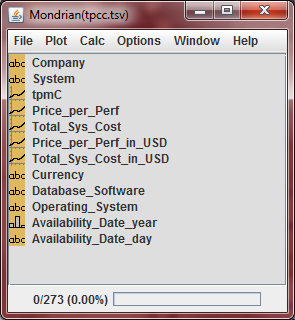
\includegraphics[width=0.30\textwidth]{figures/mondrian_tpcc_betoltve.png}
\caption{A Mondrianba betöltött adathalmaz oszlopai \label{fig:mondrian_tpcc_betoltve}}
\end{figure}

\subsection{Mely években megjelent konfigurációkat tartalmazza a benchmark? Mennyire használható/releváns napjainkban?}
\subsubsection*{Megoldás}
Válasszuk ki az \oszlopnev{Availability\_Date\_year} oszlopot, majd \menuelem{Plot $\rightarrow$ Barchart}. Látható, hogy 2009-től megfogyatkozott a feltöltött eredmények száma.

\subsection{Az egyes beszállítók mely években voltak aktívak? Mely beszállító a nagy játékos?}
\subsubsection*{Megoldás}
Válasszuk ki a \texttt{Company} oszlopot, majd Plot $\rightarrow$ Barchart. Az egyes beszállítók neveire kattintva az éveket tartalmazó ablakban láthatjuk az aktív éveket.
\subsubsection*{Megállapítások, megjegyzések}
A HP minden évben adott ki konfigurációt (kivétel 2012, de még nincs vége az évnek), az Oracle csak az utóbbi két évben.

\subsection{Ha cégünk igényeit egy alacsonyabb teljesítményű konfigurációval is ki tudjuk elégíteni, akkor mely beszállítók közül válasszunk?}
\subsubsection*{Megoldás}
Nézzük meg a tpmC eloszlását. Ehhez válasszuk ki a \texttt{tpmC} oszlopot, majd Plot $\rightarrow$ Histogram. A bal szélső oszlopra kattintva a Company nézetén láthatjuk a szóba jöhető beszállítókat. A hisztogram bin szélességét a \textit{Ctrl + UP/DOWN} billentyűkkel módosíthatjuk.
\subsubsection*{Megállapítások, megjegyzések}
A jobb szélső oszlop az Oracle csúcskategóriás klasztere.

\subsection{Mit lehet megállapítani a teljesítmény változásáról?}
\subsubsection*{Megoldás}
Válasszuk ki az \texttt{Availability\_Date\_year} vagy \texttt{Availability\_Date\_day}, majd a \texttt{tpmC} oszlopokat, Plot $\rightarrow$ Scatterplot.
\subsubsection*{Megállapítások, megjegyzések}
Látható a teljesítmény növekedése, de néhány csúcsteljesítményű szerver kivételével inkább az alsó sávban helyezkednek el. Illesszünk regressziós görbét a pontokra. Az \texttt{Availability\_Date\_year - tpmC} scatterplotra jobb gombbal kattintva smoothers $\rightarrow$ ls-line. 

\todo{RServe hiánya esetén csak ez megy}

\todo{Többi simítógörbét megmutatni}

Ha valamelyik pont fölé visszük a kurzort és közben nyomva tartjuk a Ctrl-t akkor kiírja a ponthoz tartozó értékeket.
\subsubsection*{Ugyanez Boxplot alkalmazásával}
Válasszuk ki az \texttt{Availability\_Date\_year}, majd a \texttt{tpmC} oszlopokat, Plot $\rightarrow$ Boxplot y by x. Megfigyelhető a mediánok értékének növekedése.

\subsection{Hogyan alakulnak a tranzakciós és összköltségek?}
\subsubsection*{Megoldás}
Válasszuk ki az \texttt{Availability\_Date\_year}, majd a \texttt{Price\_per\_Perf\_in\_USD} oszlopokat, Plot $\rightarrow$ Scatterplot. Ezután az \texttt{Availability\_Date\_year}, \texttt{Total\_Sys\_Cost\_in\_USD} párost hasonló módon. Tegyünk regressziós görbét az ábrákra!
\todo{Leírni, hogyan tegyük oda a görbét!}
Láthatjuk, hogy a tranzakciós költségek csökkennek, viszont a teljes költségek inkább növekednek.
\subsubsection*{Megállapítások, megjegyzések}
Ha a tpmC ábrán kijelöljük a felső néhány pontot, akkor megállapíthatjuk, hogy a teljes költségek ugyan magasak, de a teljesítmény/ár arány még mindig jónak számít.

\subsection{Milyen adatbázis-kezelő szoftvert válasszunk, ha még mindig az olcsóbb megoldást szeretnénk használni?}
\subsubsection*{Megoldás}
Válasszuk ki a \texttt{Database\_Software} oszlopot, majd Plot $\rightarrow$ Barchart. A teljes költséget ábrázoló ploton jelöljük ki az alsó pontokat.
\subsubsection*{Megállapítások, megjegyzések}
Jól látható, hogy az MS SQL-es konfigurációk inkább az alsó és középső árkategóriákat fedik le, míg a felső kategória az Oracle-re és IBM-re jellemző.

\subsection{Milyen operációs rendszert válasszunk, ha a teljes költséget minimalizálni akarjuk?}
\subsubsection*{Megoldás}
Az \texttt{Operating\_System} oszlopból készítsünk egy barchartot, majd az \texttt{Availability\_Date\_year} - \\ \texttt{Total\_Sys\_Cost\_in\_USD} scatterploton jelöljük ki az alsó pontokat. Látható, hogy főleg az MS Windows-os és Oracle Enterprise Linux-os konfigurációk a legolcsóbbak a teljes költséget nézve.
\subsubsection*{Megállapítások, megjegyzések}
Az \texttt{Availability\_Date\_year} - \texttt{tpmC} scatterploton kijelölve a felső pontokat látható, hogy a legnagyobb teljesítményt nyújtó gépeken Unix/Linux variánsok futnak, míg az \texttt{Operating\_System} barcharton a Windows-ra kattintva láthatjuk a tpmC ábráján, hogy ezen konfigurációk teljesítménye nem a legjobb.

\subsection{Melyik beszállító melyik adatbázis-kezelőben és operációs rendszerben ,,utazik''?}
\subsubsection*{Megoldás}
A már meglévő \texttt{Operating\_System}, \texttt{Database\_Software} és \texttt{Company} barchartok esetén a beszállítókat végig kattintgatva megvizsgálhatjuk, hogy mely OS-eket és DBMS-eket preferálják.

\subsection{Melyik beszállítót, adatbázis-kezelőt és operációs rendszert tartalmazza a leggyakrabban az adathalmaz?}
\subsubsection*{Megoldás}
Vegyünk fel mozaik diagramokat! Ehhez válasszuk ki a \texttt{Company} és \texttt{Database\_Software} oszlopokat, ezután Plot $\rightarrow$ Mosaic Plot, majd végezzük el ugyanezt a \texttt{Company} és \texttt{Operating\_System} oszlopokra is. A legnagyobb területű téglalapokat ki választva nézhetjük meg, hogy melyik a legelterjedtebb OS, DBMS és beszállító a piacon.
\subsubsection*{Megállapítások, megjegyzések}
A legnagyobb téglalapot a HP - MS Windows - MS SQL hármas birtokolja, ami természetesen valószínűleg nem független az elterjedtségtől sem.

\subsection{Próbáljunk összefüggést találni a teljesítmények, költségek, operációs rendszerek és adatbázis-kezelők között!}
\subsubsection*{Megoldás}
Jelöljük ki a \texttt{Company}, \texttt{tpmC}, \texttt{Price\_per\_Perf\_in\_USD}, \texttt{Total\_Sys\_Cost\_in\_USD}, \\ \texttt{Database\_Software},  \texttt{Operating\_System} és \texttt{Currency} oszlopokat, majd Plot $\rightarrow$ Parallel Coordinates.
\subsubsection*{Megállapítások, megjegyzések}
Az MSSQL fajlagosan (tmpC/USD) drága, de az összköltségük ezeknek a konfigurációknak alacsony. A Windows alapú rendszerek olcsóbbak, de rosszabb teljesítményt is nyújtanak. Az AIX operációs rendszerre csak DB2, Oracle és hatékonynak mondható adatbázis-kezelők vannak.
A párhuzamos koordináták módszere arra is alkalmas, hogy szelektáljunk a változók között. Pl. a Currency oszlopnál látszik, hogy semmihez nincs köze. Fontos a változók sorrendje (pl. \texttt{Database\_Software}, \texttt{Operating\_System} egymás mellé érdemes helyezni).

\section{Összefoglalás}

\todo{Megírni!}

\end{document}